% L7a student companion deck.
%
% The frame order mirrors the lecture notebook so students can take notes while
% the instructor works through the notebook. The disclaimer is intentionally
% slide 2, by instructor preference.
\documentclass[aspectratio=169,11pt]{beamer}
\usepackage{vnslides}

\newcommand{\E}{\mathbb{E}}
\newcommand{\bg}{\mathbf{g}}
\newcommand{\bw}{\mathbf{w}}
\newcommand{\bn}{\mathbf{n}}
\newcommand{\bal}{\boldsymbol{\alpha}}
\newcommand{\bbe}{\boldsymbol{\beta}}
\newcommand{\Tan}{\mathcal{T}}
\newcommand{\Ap}{\mathcal{A}^{+}}
\newcommand{\Am}{\mathcal{A}^{-}}
\newcommand{\Rset}{\mathcal{R}}
\newcommand{\WP}{W_{\mathcal{P}}}
\newcommand{\Wadj}{W_{\mathrm{adj}}}
\newcommand{\np}{|\mathcal P|}
\newcommand{\SigSIM}{\hat{\boldsymbol{\Sigma}}_{g,\mathrm{SIM}}}
\newcommand{\gSIM}{\hat{\bg}_{\mathrm{SIM}}}

\title{\texorpdfstring{{\vnheavy L7a}}{L7a}: Utility-Based Allocation and the Adaptive Rebalancing Engine}
\subtitle{CHEME 5660 Cornell University}
\author{Copyright Jeffrey Varner 2026. All Rights Reserved}

\begin{document}

\vntitlepage

\begin{frame}{Disclaimer and Risks}
  \vspace{0.6em}
  \textbf{\ink{Training only.}} This content is for training and informational
  purposes only. The teaching team does not make, give, or endorse any offer or
  solicitation to buy or sell securities or derivative products, or provide
  investment or trading advice or strategy.

  \vspace{1.1em}
  \textbf{\ink{Risk.}} Trading involves risk and is generally not recommended for
  those with limited resources, experience, or a low risk tolerance. Past
  performance does not guarantee future success.

  \vspace{1.1em}
  \textbf{\ink{Responsibility.}} You are responsible for your investment decisions
  based on your financial circumstances, objectives, risk tolerance, and
  liquidity needs.
\end{frame}

\begin{frame}{Objectives for Today}
  Today we stop treating a portfolio as a vector of weights chosen once and treat
  it as a process: preferences computed every day from the single index model and
  the state of the market, answering which assets belong in the basket and how
  much of each, and a rebalancing engine with an account, rules, and a scorecard.

  \vspace{0.6em}
  {\large\textbf{\ink{Today's concepts}}}
  \vspace{0.2em}
  \begin{itemize}\setlength{\itemsep}{0.45em}
    \item \hilite{Why a static allocation fails}: how buy-and-hold weights drift
      with prices and how to measure it, and the three ways the minimum-variance
      inputs let the optimizer down.
    \item \hilite{Utility-based allocation}: the budget-constrained problem, the
      Cobb--Douglas closed form, CES and its three limits, and preference weights
      from the SIM and two market inputs: signs choose the basket, magnitudes the
      weights.
    \item \hilite{The rebalancing engine}: a self-financing account with costs,
      next-bar execution, three trigger rules, and how to score a realized path.
  \end{itemize}
\end{frame}

\begin{frame}{Lectures and Examples}
  \vspace{0.3em}
  {\normalsize\textbf{\ink{Lecture:}}\par
  \dimmed{CHEME-5660-L7a-Lecture-Utility-Allocation-Rebalancing-Fall-2026.ipynb}}

  \vspace{0.6em}
  {\normalsize\textbf{\ink{Example 1:}}\par
  \dimmed{CHEME-5660-L7a-Example-Utility-Allocator-Fall-2026.ipynb}}

  \vspace{0.6em}
  {\normalsize\textbf{\ink{Example 2:}}\par
  \dimmed{CHEME-5660-L7a-Example-Adaptive-Rebalancing-Scorecard-Fall-2026.ipynb}}

  \vspace{0.6em}
  {\normalsize\textbf{\ink{Example 3:}}\par
  \dimmed{CHEME-5660-L7a-Example-Portfolio-Drift-Fall-2026.ipynb}}

  \vspace{0.5em}
  The first example builds the allocator and reads which firms belong in the
  basket; the second runs the engine through 2025 against buy-and-hold baselines;
  the third measures the drift of a tangent portfolio held through the year.
\end{frame}

% ==== concept review =========================================
\begin{frame}{Concept Review: Allocation as a Time-Stamped Decision}
  L5b and L6b chose weights $\bw$ over $\np$ risky assets from an expected
  growth-rate vector and a growth-rate covariance; with the SIM of L6a those inputs
  are $\gSIM=\hat{\bal}+\hat{\bbe}\,g'_M$ and
  $\SigSIM=s^2_{g,M}\hat{\bbe}\hat{\bbe}^{\top}+\hat{\mathbf D}_g$ ($g'_M$,
  $s^2_{g,M}$ the training-period market mean and variance; $\hat{\mathbf D}_g$ the
  diagonal matrix of residual variances).
  \begin{itemize}\setlength{\itemsep}{0.3em}
    \item Target $g_\star$: $\bw(g_\star)$ minimizes $\bw^{\top}\hat{\Sigma}_g\bw$
      subject to $\bw^{\top}\hat{\bg}=g_\star$, $\mathbf 1^{\top}\bw=1$, $w_i\ge0$;
      the lowest point is $\bw_{\mathrm{GMV}}$; with a risk-free asset earning
      $g_f$, the fully invested point of the ray is the tangent portfolio $\bw_{\Tan}$.
    \item Implemented on the decision date $t=0$ by buying share counts, and held:
  \end{itemize}
  \[
    n_i=\frac{w_i\,\WP(0)}{S_i(0)},\qquad
    \WP(t)=\sum_{i\in\mathcal P}n_i\,S_i(t)
  \]
  \hilite{Two things to say out loud}: the weights are optimal on the decision
  date, for the inputs estimated on that date; and the only decision the investor
  ever made was the one at $t=0$. Today is about the other days.
\end{frame}

% ==== why static fails =======================================
\begin{frame}{Why Static Allocation Fails: Mechanical Drift}
  With fixed share counts (no cash, no dividends), $w_i(t)=n_iS_i(t)/\WP(t)$; with
  $n_i=w_i(0)\WP(0)/S_i(0)$ the initial wealth cancels:
  \[
    w_i(t)=\frac{w_i(0)\,\overbrace{\bigl(S_i(t)/S_i(0)\bigr)}^{\text{price relative}}}
      {\sum_{j\in\mathcal P}w_j(0)\bigl(S_j(t)/S_j(0)\bigr)}
  \]
  Weights stay put only if every held asset has the same price relative, which
  does not happen in practice. The drift on day $t$ is the half-$L^1$ distance,
  the fraction of wealth a rebalance back to $w_i(0)$ would trade (before costs):
  \[
    \tfrac12\sum_{i\in\mathcal P}\lvert w_i(t)-w_i(0)\rvert
  \]
  \slidenote{Example 3 (SIM tangent portfolio through 2025: drift $4.6\%$ by year end):}{\dimmed{CHEME-5660-L7a-Example-Portfolio-Drift-Fall-2026.ipynb}}
\end{frame}

\begin{frame}{Why Static Allocation Fails: Fragile Inputs}
  Drift is the benign failure; the optimizer's inputs are the serious one. Three
  tendencies of estimated minimum-variance and tangent portfolios recur:
  \begin{itemize}\setlength{\itemsep}{0.45em}
    \item \hilite{Input sensitivity}: estimated inputs are treated as exact, so
      estimation errors move the weights; the tangent portfolio overweights assets
      whose growth is overstated (Michaud's \emph{error maximizer}, 1989), and
      errors in the means matter far more than errors in the variances (Chopra and
      Ziemba, 1993).
    \item \hilite{Concentration}: without binding constraints the tangent
      portfolio, and often the GMV portfolio, holds a few names (four of thirteen
      in L6b).
    \item \hilite{Assumption fragility}: one stable distribution is assumed, but
      correlations rise and volatilities jump in the episodes that matter.
  \end{itemize}
  Two responses: change the \hilite{objective}, writing preferences for each
  asset explicitly and letting them respond to the market state (today); or
  update the \hilite{inputs} as data arrive (L7b).
\end{frame}

% ==== utility maximization ===================================
\begin{frame}{Utility Maximization}
  Instead of the smallest variance for a target, ask a consumer-choice question:
  given a budget and today's market, which portfolio does the investor prefer
  most? A utility function ranks portfolios, larger for more preferred. At time
  $t$, with prices $S_i(t)$ (USD per share) and wealth $\WP(t)$ (USD), choose the
  share counts $n_i\ge0$:
  \[
    \boxed{\operatorname*{maximize}_{n_1,\ldots,n_{\np}}\;U(n_1,\ldots,n_{\np})
      \qquad\text{subject to}\qquad\sum_{i\in\mathcal P}n_i\,S_i(t)=\WP(t)}
  \]
  \begin{itemize}\setlength{\itemsep}{0.35em}
    \item A \hilite{holding utility}: a preference over the shares held today at
      today's prices, not the expected utility of an uncertain terminal wealth;
      risk enters through the preferences and the engine's rules.
    \item \hilite{Two coupled questions}: which assets belong in the basket today,
      and how much of each. The utility functions answer the second; the
      preference model answers the first. Both are recomputed every trading day.
  \end{itemize}
\end{frame}

\begin{frame}{Cobb--Douglas Utility: Sign Classifies, Magnitude Allocates}
  Let $\gamma_i\in(-1,1)$ be the preference weight of asset $i$. Its \hilite{sign}
  splits the assets into the preferred set $\Ap=\{i:\gamma_i>0\}$, the basket, and
  the non-preferred set $\Am=\{i:\gamma_i\le0\}$, held at a floor of $n_{\min}\ge0$
  shares each; the utility is a product of powers over the preferred set,
  $U=\prod_{i\in\Ap}n_i^{\gamma_i}$ ($n_i>0$ on $\Ap$, $n_i=n_{\min}$ on $\Am$).
  With $\Wadj=\WP(t)-n_{\min}\sum_{k\in\Am}S_k(t)>0$ the budget left after the
  floors and at least one preferred asset, the maximizer is closed form:
  \[
    \boxed{n_i^\star=\underbrace{\frac{\gamma_i}{\sum_{j\in\Ap}\gamma_j}}_{\text{preference share}}
      \cdot\underbrace{\frac{\Wadj}{S_i(t)}}_{\text{budget in shares}}\quad(i\in\Ap),
      \qquad n_i^\star=n_{\min}\quad(i\in\Am)}
  \]
  The \hilite{dollar weight} of a preferred asset within the preferred budget is
  its normalized preference weight $\gamma_i/\sum_{j\in\Ap}\gamma_j$, independent
  of prices (times $\Wadj/\WP(t)$ as a fraction of total wealth). An empty basket
  means floors plus cash.
\end{frame}

\begin{frame}{Cobb--Douglas Utility: Derivation}
  Maximizing $U$ over $\Ap$ is maximizing $\ln U=\sum_{i\in\Ap}\gamma_i\ln n_i$
  (the log is increasing). With multiplier $\lambda$ on the budget over the
  preferred set, the first-order condition for asset $i$ is:
  \[
    \frac{\gamma_i}{n_i}=\lambda\,S_i(t)\qquad\Longleftrightarrow\qquad
    \underbrace{n_iS_i(t)}_{\text{dollars in }i}=\frac{\gamma_i}{\lambda}
  \]
  Each preferred asset receives dollars in proportion to its exponent. Summing
  over $\Ap$ gives $\Wadj=\sum_{j\in\Ap}\gamma_j/\lambda$, and substituting back
  gives the boxed result; strict concavity of $\ln U$ on the positive orthant
  makes it the unique maximum.
  \begin{itemize}\setlength{\itemsep}{0.35em}
    \item The closed form applies to the preferred set only: a non-positive
      $\gamma_i$ is a classification, not an exponent to insert (for $\gamma_i<0$
      the term $n_i^{\gamma_i}$ blows up as $n_i\downarrow0$).
    \item The allocation responds immediately to a change in the preferences: no
      covariance matrix, no quadratic program, no numerical solver.
  \end{itemize}
\end{frame}

\begin{frame}{CES Utility: A Concentration Dial}
  For an elasticity of substitution $\eta>0$, $\eta\ne1$, the CES utility over the
  preferred set is $U_{\mathrm{CES}}(\bn)=\bigl(\sum_{i\in\Ap}\gamma_i\,n_i^{(\eta-1)/\eta}\bigr)^{\eta/(\eta-1)}$
  ($\gamma_i$ now a coefficient). Its maximizer is closed form, share counts
  proportional to the bang for the buck raised to $\eta$:
  \[
    \boxed{n_i^\star=\Wadj\;\frac{\bigl(\gamma_i/S_i(t)\bigr)^{\eta}}
      {\sum_{j\in\Ap}S_j(t)\bigl(\gamma_j/S_j(t)\bigr)^{\eta}}\quad(i\in\Ap)}
  \]
  \begin{itemize}\setlength{\itemsep}{0.3em}
    \item $\eta\to1$: the Cobb--Douglas allocation (its limit). \ $\eta\to\infty$:
      all of the preferred budget on the largest $\gamma_i/S_i(t)$ (when unique).
      \ $\eta\to0^+$: equal share counts of every preferred asset.
    \item Engine's CES variant: $\eta(\xi_t)=\eta_{\min}+(\eta_{\max}-\eta_{\min})/(1+|\xi_t|)$,
      $0<\eta_{\min}\le\eta_{\max}$ ($0.5$, $5$ in the examples): concentrate when
      the market-state signal $\xi_t$ (an EMA crossover, two frames on) is quiet,
      diversify when it is loud.
      Proofs, log-linear utility, and a share-denomination caveat: advanced notebook.
  \end{itemize}
\end{frame}

% ==== preference weights =====================================
\begin{frame}{Preference Weights from the Single Index Model}
  From the SIM parameters $(\alpha_i,\beta_i)$ and two market inputs on day $t$,
  the recent market growth rate $\tilde g_{M,t}$ and a market-state signal $\xi_t$:
  \[
    \boxed{\gamma_i(t)=\tanh\!\left(\frac{\alpha_i}{\beta_i^{\xi_t}}+\beta_i^{1-\xi_t}\,\tilde g_{M,t}\right)}
  \]
  The $\tanh$ bounds the weight in $(-1,1)$. Its argument is the SIM's expected
  growth of asset $i$ in today's market, $\alpha_i+\beta_i\tilde g_{M,t}$ (inverse
  years), through a \hilite{regime lens}: it equals $(\alpha_i+\beta_i\tilde g_{M,t})/\beta_i^{\xi_t}$.
  \begin{itemize}\setlength{\itemsep}{0.3em}
    \item \hilite{Which assets belong in the basket}: $\beta_i^{\xi_t}>0$ and
      $\tanh$ keeps sign, so $\operatorname{sign}\gamma_i(t)=\operatorname{sign}(\alpha_i+\beta_i\tilde g_{M,t})$:
      preferred exactly when $\tilde g_{M,t}>-\alpha_i/\beta_i$. The signal never
      changes the classification; the recent market growth does.
    \item \hilite{How much of each}: the lens moves the magnitudes: bearish
      ($\xi_t>0$) tilts toward low-beta names, bullish ($\xi_t<0$) toward high-beta.
  \end{itemize}
\end{frame}

\begin{frame}{Preference Weights: The Basket, and Assumptions Stated}
  \begin{itemize}\setlength{\itemsep}{0.45em}
    \item As $\tilde g_{M,t}$ moves, assets \hilite{cross between the sets}: a
      strong market pulls in firms with a small negative $\alpha_i$ and a large
      $\beta_i$; a weak market pushes out everything but the strongest intercepts.
    \item If every $\gamma_i(t)\le0$, the model is saying \hilite{this basket does
      not belong in this market}: the allocator holds the floors plus cash, and an
      investor not content with cash should rethink which assets are in the
      basket (the ticker-picking methods of L12b and L13a; L7b's parameter
      updates move the thresholds too).
    \item \hilite{Assumptions}: (i) $\beta_i>0$ (the course firms: $0.54$ to
      $1.75$, asserted; a non-positive beta needs a rule, e.g., assign to $\Am$);
      (ii) the argument is an annualized growth rate read as a pure number at the
      one-year horizon; (iii) $\tilde g_{M,t}$ swings by about a unit per year, an
      order of magnitude more than the intercepts: that is what makes the basket
      respond, and why the schedule and rules decide how often it is acted on.
  \end{itemize}
\end{frame}

\begin{frame}{The Market Inputs}
  Both come from SPY with exponential moving averages, $\bar S_t=\omega S_t+(1-\omega)\bar S_{t-1}$,
  $\omega=2/(L+1)$, window $L$ days. With $L_{\mathrm{short}}=21$, $L_{\mathrm{long}}=63$,
  and a dimensionless gain $G>0$, the signal is the scaled crossover:
  \[
    \boxed{\xi_t=-G\left(\frac{\bar S^{\mathrm{short}}_t}{\bar S^{\mathrm{long}}_t}-1\right)}
  \]
  \begin{itemize}\setlength{\itemsep}{0.25em}
    \item Falling market (short EMA below long): $\xi_t>0$, bearish; rising:
      $\xi_t<0$, bullish; $G$ sets $|\xi_t|\le1$ on 99\% of training days ($G\approx21$).
    \item $\tilde g_{M,t}$: the EMA (window $L_{\mathrm{growth}}=10$) of the daily
      market growth rates $g_{M,t}=\ln(S_t/S_{t-1})/\Delta t$.
      \hilite{Both inputs on day $t$ use prices through day $t-1$.}
  \end{itemize}
  \slidenote{Example 1:}{\dimmed{CHEME-5660-L7a-Example-Utility-Allocator-Fall-2026.ipynb} (first trading day of 2025: $\tilde g_M=-0.76$ per year, no firm preferred)}
\end{frame}

% ==== engine ================================================
\begin{frame}{The Rebalancing Engine}
  \vspace{-0.3em}
  \begin{center}
    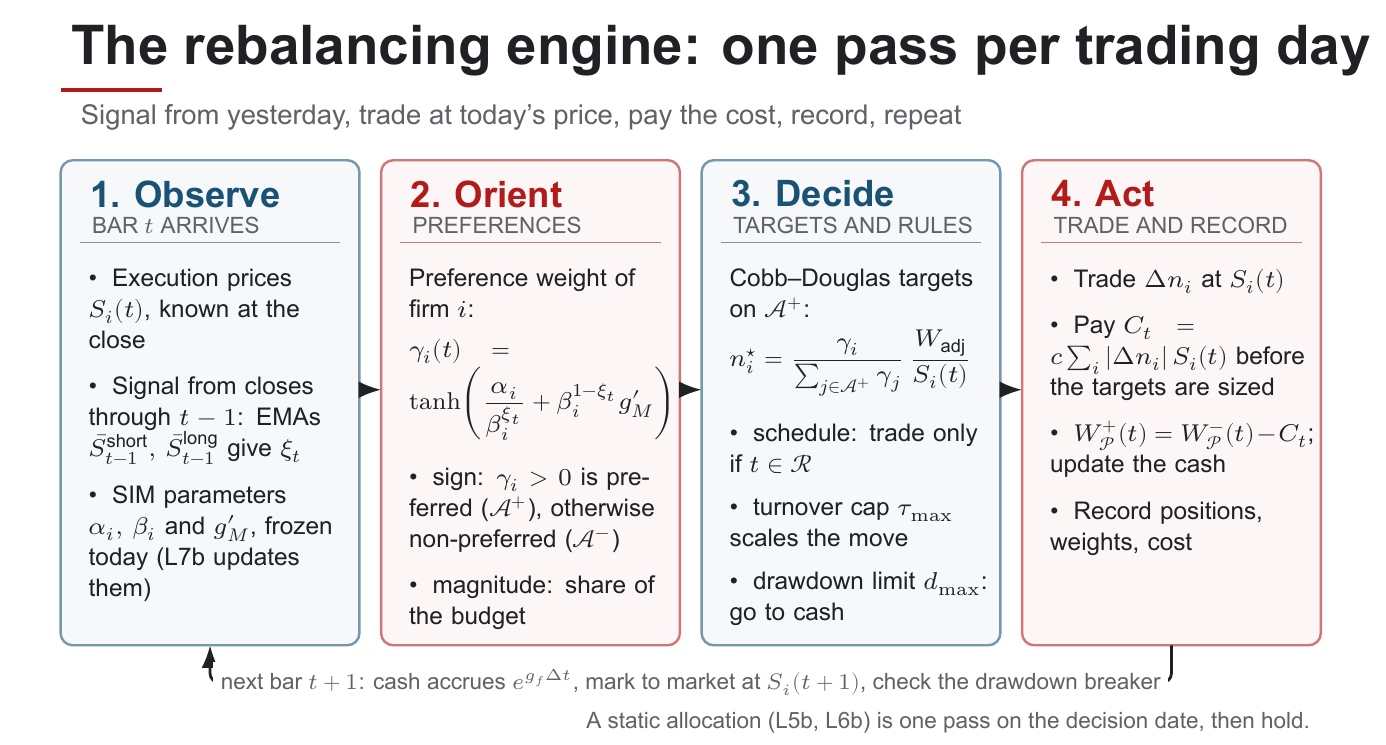
\includegraphics[height=0.72\textheight,keepaspectratio]{../figs/Fig-L7a-Rebalancing-Engine-Loop.png}
  \end{center}
  \vspace{-0.5em}
  Every trading day is one pass: observe, orient, decide, act. A static
  allocation is one pass on the decision date, then nothing.
\end{frame}

\begin{frame}{The Rebalancing Engine: The Account and the Timing}
  Let $n_{i,t}$ be the shares held after the close of day $t$; cash earns $g_f$.
  At the close of day $t$, before any trade, the book is worth:
  \[
    W^-_{\mathcal P}(t)=\underbrace{\mathrm{cash}_{t-1}\,e^{g_f\Delta t}}_{\text{cash}}
      +\underbrace{\textstyle\sum_{i}n_{i,t-1}\,S_i(t)}_{\text{marked to market}}
  \]
  Trading share deltas $\Delta n_i$ at the close $S_i(t)$ moves gross notional
  $Q_t=\sum_i|\Delta n_i|S_i(t)$ and costs $C_t=c\,Q_t$ ($c$ the cost rate). The
  cost comes out of the book and the positions are sized against what is left,
  the two solved together:
  \[
    \boxed{W^+_{\mathcal P}(t)=W^-_{\mathcal P}(t)-C_t}
  \]
  so $\mathrm{cash}_t+\sum_in_{i,t}S_i(t)=W^+_{\mathcal P}(t)$ exactly and cash
  never goes negative. \hilite{Next-bar execution}: inputs and preferences for
  day $t$ use prices through $t-1$; the trade executes at day $t$'s close (market
  on close). A close-based signal traded at that close is look-ahead; Example 2
  asserts the lag in code.
\end{frame}

\begin{frame}{The Rebalancing Engine: Three Trigger Rules}
  Three rules bound the loop (else it trades daily, ignores a crash, or acts on
  every wiggle of the inputs):
  \begin{itemize}\setlength{\itemsep}{0.25em}
    \item \hilite{Reallocation schedule} $\Rset$: trade only on days $t\in\Rset$
      (daily, or every 21 days); hold otherwise.
    \item \hilite{Turnover cap} $\tau_{\max}$: with $\Delta w_i$ the change of
      asset $i$'s weight and $\Delta w_{\mathrm{cash}}=-\sum_i\Delta w_i$, the
      one-way turnover $\tau_t=\tfrac12\bigl(\sum_i|\Delta w_i|+|\Delta w_{\mathrm{cash}}|\bigr)$
      is the fraction of wealth that changes hands one way; a move with
      $\tau_t>\tau_{\max}$ is scaled down (the cost applies to the gross $Q_t$).
    \item \hilite{Drawdown limit} $d_{\max}$: a circuit breaker checked every day
      before the schedule; if $1-W^-_{\mathcal P}(t)/\max_{s\le t}W^-_{\mathcal P}(s)>d_{\max}$,
      liquidate to cash (bypassing the cap), stay in cash $n_{\mathrm{lock}}$ more
      days, rebase the peak on the first scheduled trade after. It does not cap the
      recorded drawdown at $d_{\max}$.
  \end{itemize}
  They interact: all-cash to fully invested is a one-way turnover of one, so with
  $\tau_{\max}=0.5$ the engine is only half invested until its next scheduled day.
\end{frame}

\begin{frame}{Algorithm: Rebalancing Engine (Backtest), Setup}
  The engine is \hilite{allocator-agnostic}: it takes the prices and a target
  function, and our target functions wrap the allocators of this lecture around
  the lagged preference weights.
  \begin{itemize}\setlength{\itemsep}{0.45em}
    \item \textbf{\ink{Given:}} close prices $S_i(t)$, $t=1,\ldots,N$; the initial
      wealth $\WP(0)$ in cash; the set $\Rset$; the rule parameters
      $(c,\tau_{\max},d_{\max},n_{\mathrm{lock}})$.
    \item \textbf{\ink{Target function}} $\bw^\star(t,\mathrm{state})$: returns
      risky weights ($w_i^\star\ge0$, $\sum_iw_i^\star\le1$, remainder cash) from
      the day and the current state (pre-trade wealth, weights, shares, cash, and a
      copy of the day's execution prices).
    \item \textbf{\ink{Ours:}} compute $\gamma_i(t)$ from the market inputs through
      $t-1$, allocate by Cobb--Douglas (or CES with $\eta(\xi_t)$) at the day's
      prices, return the allocation as weights; on an empty basket, floors plus cash.
    \item \textbf{\ink{Static baselines:}} the same loop with a constant target and
      $\Rset=\{1\}$: same costs, same accounting.
  \end{itemize}
\end{frame}

\begin{frame}{Algorithm: Rebalancing Engine (Backtest), Daily Loop}
  \textbf{\ink{For $t=1,\ldots,N$}} (one bar at a time, under the timing rule):
  \begin{enumerate}\setlength{\itemsep}{0.1em}
    \item Accrue cash by $e^{g_f\Delta t}$; mark to market at $S_i(t)$ to get
      $W^-_{\mathcal P}(t)$; update the running peak.
    \item Breaker: if the drawdown exceeds $d_{\max}$ with risky positions held,
      liquidate at $S_i(t)$, pay $c$ on the notional sold, lock $n_{\mathrm{lock}}$
      more days, go to 5.
    \item If $t\in\Rset$ and not locked: ask for $\bw^\star$ (rebase the peak after
      a lock); form the proposed change of weights, scale to $\tau_{\max}$.
    \item Solve cost and positions together on the post-cost budget; execute
      $\Delta n_i$ at $S_i(t)$; pay $C_t=c\,Q_t$; update the cash.
    \item Record wealth, cash, positions, weights, turnover, cost, flags: the
      histories every scorecard consumes.
  \end{enumerate}
  \slidenote{Example 2:}{\dimmed{CHEME-5660-L7a-Example-Adaptive-Rebalancing-Scorecard-Fall-2026.ipynb}}
\end{frame}

% ==== scoring ===============================================
\begin{frame}{Scoring a Realized Path}
  Did the portfolio beat what the same dollars earn at the risk-free growth rate?
  For one outflow, one terminal value, constant $g_f$, horizon $T=N\Delta t$ years:
  \[
    \boxed{\mathrm{NPV}(g_f,T)=\underbrace{-\WP(0)}_{\text{investment}}
      +\underbrace{\WP(T)\,e^{-g_fT}}_{\text{discounted terminal wealth}}}
  \]
  positive means the run beat cash at $g_f$; the risk-free portfolio is the zero.
  \begin{itemize}\setlength{\itemsep}{0.2em}
    \item \hilite{Realized growth} $\ln(\WP(T)/\WP(0))/T$; \hilite{maximum drawdown}
      $\max_t\bigl(1-\WP(t)/\max_{s\le t}\WP(s)\bigr)$.
    \item \hilite{Realized Sharpe ratio}: mean of the daily excess log growth over
      its standard deviation, times $\sqrt{1/\Delta t}$ (annualized, as in L6b).
    \item \hilite{Turnover, cost, interventions}: $\sum_t\tau_t$, $\sum_tC_t$,
      breaker firings.
  \end{itemize}
  One row per run, these columns. \hilite{One path is one draw}: what each policy
  did, not how likely it was; fail rates and tail quantiles need many paths (L7b).
\end{frame}

\begin{frame}{Scoring a Realized Path: 2025 in One Table}
  Example 2: $\Rset$ every 21 days, $\tau_{\max}=0.5$, $d_{\max}=0.10$, $c=5$
  basis points, one engine for every run. The model emptied the basket on 57 of
  250 days and preferred all thirteen firms on 152.
  \begin{itemize}\setlength{\itemsep}{0.35em}
    \item \hilite{Cobb--Douglas, monthly}: 12 scheduled trades, floors plus cash on
      50 days, no breaker firing; ended at $1.53$ times initial wealth, drawdown
      $9.0\%$ (rules off: $1.52$).
    \item \hilite{Cobb--Douglas, daily}: 228 trades, one breaker firing, twenty
      times the cost; $1.40$ ($10.8\%$). \hilite{CES with $\eta(\xi_t)$, monthly}:
      $1.29$ ($9.2\%$).
    \item \hilite{Buy and hold}: tangent $1.28$ (drawdown $31\%$), GMV $1.38$
      ($13\%$), equal weights $1.59$ ($24\%$), SPY $1.17$ ($19\%$).
  \end{itemize}
  Read across, then against the baselines: who beat cash, what the basket
  selection did on the bad days, what a schedule cost. One year, one draw.
  \slidenote{Example 2:}{\dimmed{CHEME-5660-L7a-Example-Adaptive-Rebalancing-Scorecard-Fall-2026.ipynb}}
\end{frame}

% ==== optional advanced material =============================
\begin{frame}{Optional Advanced Material}
  \vspace{0.4em}
  {\normalsize\textbf{\ink{Advanced:}} \dimmed{advanced/adaptive\_utility/}\par
  \dimmed{CHEME-5660-L7a-Advanced-CES-Limits-Fall-2026.ipynb}}

  \vspace{0.7em}
  Optional, not a prerequisite for L7b. Derives the CES closed form and proves its
  three limits (Cobb--Douglas at $\eta\to1$, concentration at $\eta\to\infty$,
  equal share counts at $\eta\to0^+$), reads the two limits of the elasticity
  rule $\eta(\xi_t)$, shows that log-linear utility has the Cobb--Douglas
  optimizer, and shows why the CES allocation over share counts depends on the
  price level of each share when $\eta\ne1$.
  \slidenote{Notebook:}{\href{https://github.com/varnerlab/CHEME-5660-CourseRepository-Fall-2026/tree/main/lectures/week-7/L7a/advanced}{lectures/week-7/L7a/advanced}, also linked from the lecture notebook.}
\end{frame}

\begin{frame}{Summary}
  Today: drift and fragile inputs, the Cobb--Douglas and CES allocators,
  preferences from the SIM and two market inputs, and an engine with an account,
  rules, and a scorecard.

  {\large\textbf{\ink{Key takeaways}}}
  \begin{itemize}\setlength{\itemsep}{0.1em}
    \item \hilite{Utility makes preferences explicit, Cobb--Douglas turns them
      into weights in closed form}: sign puts an asset in or out of the basket,
      magnitude sets its share of the preferred budget; CES is a concentration dial.
    \item \hilite{The SIM plus two market inputs supplies the preferences, the
      rules bound the response}: recent market growth chooses the basket (empty
      means rethink it, or hold cash), the signal tilts the magnitudes; the rules
      decide when, how far, and whether to act.
    \item \hilite{A realized-path scorecard is one draw}: NPV against cash,
      drawdown, growth, Sharpe, turnover, cost say what happened; the distribution
      needs many paths.
  \end{itemize}
  Next, L7b: SIM parameters that update as data arrive, and an ensemble of futures.
\end{frame}

\transitionframe{Today: preferences computed every day, an allocation in closed form, and an engine that pays its own costs.}

\end{document}
